\documentclass[]{article}
\usepackage{lmodern}
\usepackage{amssymb,amsmath}
\usepackage{ifxetex,ifluatex}
\usepackage{fixltx2e} % provides \textsubscript
\ifnum 0\ifxetex 1\fi\ifluatex 1\fi=0 % if pdftex
  \usepackage[T1]{fontenc}
  \usepackage[utf8]{inputenc}
\else % if luatex or xelatex
  \ifxetex
    \usepackage{mathspec}
  \else
    \usepackage{fontspec}
  \fi
  \defaultfontfeatures{Ligatures=TeX,Scale=MatchLowercase}
\fi
% use upquote if available, for straight quotes in verbatim environments
\IfFileExists{upquote.sty}{\usepackage{upquote}}{}
% use microtype if available
\IfFileExists{microtype.sty}{%
\usepackage{microtype}
\UseMicrotypeSet[protrusion]{basicmath} % disable protrusion for tt fonts
}{}
\usepackage[margin=1in]{geometry}
\usepackage{hyperref}
\hypersetup{unicode=true,
            pdftitle={BEE2038 - Second tutorial - Instructor's guide},
            pdfborder={0 0 0},
            breaklinks=true}
\urlstyle{same}  % don't use monospace font for urls
\usepackage{graphicx,grffile}
\makeatletter
\def\maxwidth{\ifdim\Gin@nat@width>\linewidth\linewidth\else\Gin@nat@width\fi}
\def\maxheight{\ifdim\Gin@nat@height>\textheight\textheight\else\Gin@nat@height\fi}
\makeatother
% Scale images if necessary, so that they will not overflow the page
% margins by default, and it is still possible to overwrite the defaults
% using explicit options in \includegraphics[width, height, ...]{}
\setkeys{Gin}{width=\maxwidth,height=\maxheight,keepaspectratio}
\IfFileExists{parskip.sty}{%
\usepackage{parskip}
}{% else
\setlength{\parindent}{0pt}
\setlength{\parskip}{6pt plus 2pt minus 1pt}
}
\setlength{\emergencystretch}{3em}  % prevent overfull lines
\providecommand{\tightlist}{%
  \setlength{\itemsep}{0pt}\setlength{\parskip}{0pt}}
\setcounter{secnumdepth}{0}
% Redefines (sub)paragraphs to behave more like sections
\ifx\paragraph\undefined\else
\let\oldparagraph\paragraph
\renewcommand{\paragraph}[1]{\oldparagraph{#1}\mbox{}}
\fi
\ifx\subparagraph\undefined\else
\let\oldsubparagraph\subparagraph
\renewcommand{\subparagraph}[1]{\oldsubparagraph{#1}\mbox{}}
\fi

%%% Use protect on footnotes to avoid problems with footnotes in titles
\let\rmarkdownfootnote\footnote%
\def\footnote{\protect\rmarkdownfootnote}

%%% Change title format to be more compact
\usepackage{titling}

% Create subtitle command for use in maketitle
\providecommand{\subtitle}[1]{
  \posttitle{
    \begin{center}\large#1\end{center}
    }
}

\setlength{\droptitle}{-2em}

  \title{BEE2038 - Second tutorial - Instructor's guide}
    \pretitle{\vspace{\droptitle}\centering\huge}
  \posttitle{\par}
    \author{}
    \preauthor{}\postauthor{}
    \date{}
    \predate{}\postdate{}
  

\begin{document}
\maketitle

\hypertarget{overview}{%
\section{Overview}\label{overview}}

I proposed we cover material from the
\href{https://vle.exeter.ac.uk/pluginfile.php/1435123/mod_resource/content/1/_book/ps.html\#mock-mid-term-exam}{Mock
midterm exam}.

I asked students to give me feedback on which they wanted covered but I
haven't heard from them yet. Thus I suggest we:

\begin{itemize}
\item
  ask the students at the beginning of tutorial, and let's be prepared
  to discuss ANY of these,
\item
  make sure to involve the students\ldots{} go around the room and ask
  them to answer pieces of the question (or discuss individual answer
  choices); engage them in the logic,
\item
  make the logic and the marking for the MCQ's clear.
\end{itemize}

\emph{Below I also highlight the questions I would focus on if the
students don't have strong opinions}.

\hypertarget{questions-to-focus-on}{%
\section{Questions to focus on}\label{questions-to-focus-on}}

@ref(supplycurve) : Maybe take 5 minutes max. The key insight is that we
need a constant supply curve and a shifting demand curve to observe and
estimate the former.

\hypertarget{mock-exam-with-instructor-guidelines}{%
\section{Mock exam, with instructor
guidelines}\label{mock-exam-with-instructor-guidelines}}

\hypertarget{section}{%
\subsubsection{}\label{section}}

Choose ONE. Which of the following best represents `repeated
cross-sectional firm-level micro-data that may be used to test whether
firms that engage in CSR (corporate social responsibility) activities
tend to be in more heavily-regulated industries'?

\begin{enumerate}
\def\labelenumi{\Alph{enumi}.}
\item
  A table of the average number of employees engaged in CSR per firm,
  estimates of the regulatory involvment, and amount spent on political
  lobbying in 2017, aggregated across the largest employment sectors:
  professional services, manufacturing, and retail.
\item
  A data set with ten observations, one for each of the years 2010-2018
  for a single small firm. Each observation (row) contains ten variables
  (columns) detailing the CSR expenditure, profit, and estimated
  regulatory burden for this firm, based on a survey on their CSR
  activities and spending, cross-checked against their public financial
  reportings.
\item
  A dataset of US firms between the years 1990-2015. Each year a
  different representative sample of 1000 firms are chosen and given a
  survey on their CSR activities and spending, cross-checked against
  their public financial reportings. Each firm's 4-digit SIC industry
  code is reported and merged to an independent measure of regulatory
  burden by industry by year.
\item
  A dataset of individual tax reportings (income, asset balances and
  liabilities, corporate taxes paid, dividends paid, inventory
  depreciation, loan interest, salaries and national insurance payments,
  and tax-favored capital investment and research) from all small UK
  firms between the years 1950-2015.
\item
  An excerpt of the findings from a report on the tax and regulatory
  burden and CSR activities of EU-based firms between 1970 and 2015.
\end{enumerate}

Correct: C. A dataset of US firms between the years 1990-2015. Each year
a different representative sample of 1000 firms are chosen and given a
survey on their CSR activities and spending, cross-checked against their
public financial reportings. Each firm's 4-digit SIC industry code is
reported and merged to an independent measure of regulatory burden by
industry by year.

Note, the other choices depict, respectively: a. aggregated data (not
micro-data, not firm-level data) b. a panel dataset not repeated
cross-section. Also not particular useful for testing this relationship;
one firm will not lead to any variation in `which industry' d.~Panel
data. More importantly, it doesn't seem to have any information on CSR
or on regulatory burden. e. This is a *report* not data.

By the way, note that the question about CSR is not a `causal question';
just a question about an observed relationship.

\BeginKnitrBlock{gtatip}

\textbf{Instructors}: this is a challenge question. Students may wonder
`how was I supposed to know this'? In response, point out that
`understanding data and how economists use it' was discussed in the
latter part of the `math tools' section of the web book, and in
suggested readings linked within this.

\EndKnitrBlock{gtatip}

\hypertarget{section-1}{%
\subsubsection{}\label{section-1}}

\emph{(Choose ONE)} Which of the following fields of Economics typically
uses the most pure mathematics?

\begin{enumerate}
\def\labelenumi{\Alph{enumi}.}
\item
  Applied microeconomics
\item
  Empirical labour economics
\item
  Microeconomic theory
\item
  Macroeconomics of growth
\item
  Development economics
\end{enumerate}

Microeconomic theory. Although you may be used to thinking of `theory'
as a bunch of woolly verbiage, in Economics it involves very formal
mathematics (especially Real Analysis) and logic.

\hypertarget{supplycurve}{%
\subsubsection{(Estimating a supply curve)}\label{supplycurve}}

\emph{(Choose all that are correct, and no more.)} Suppose we observe
prices and quantities traded in a market over a period of time. In such
a case, fitting a line through these points will provide a reasonable
valid estimate of a market \emph{supply} curve... (Choose ALL that are
\emph{necessary} for this.)

\begin{enumerate}
\def\labelenumi{\Alph{enumi}.}
\item
  if the supply curve was constant over this period.
\item
  if this was a period when the demand curve was constant and the supply
  curve was shifting.
\item
  if this data pertains to several dissimilar products, and we cannot
  separate these products in the data set.
\item
  if the demand curve shifted over this period.
\item
  if the supply curve is approximately linear.
\end{enumerate}

TRUE: a. if the supply curve was constant over this period.

\begin{enumerate}
\def\labelenumi{\alph{enumi}.}
\setcounter{enumi}{3}
\item
  if the demand curve shifted over this period.
\item
  if the supply curve is approximately linear.
\end{enumerate}

False:

``if this was a period when the demand curve was constant and the supply
curve was shifting.'' --- this is a condition for estimating a
\emph{demand} curve not a supply curve.

``if this data pertains to several dissimilar products, and we cannot
separate these products in the data set.'' ---With several unrelated
products it is unclear what this relationship would be depicting

\hypertarget{section-2}{%
\subsubsection{}\label{section-2}}

\emph{Choose ONE.} Suppose that, over a number of years, a country
randomly (by lottery) selected people from an eligible pool to attend
university, and all who were selected attended university, and all who
were not selected did not attend any university. Suppose that, for this
country, on average those who attended university earned significantly
more than those who did not. In such a case, which of the following
statements is most correct?

\begin{enumerate}
\def\labelenumi{\Alph{enumi}.}
\item
  This offers no valid evidence on the income returns to education
  because correlation is not causation.
\item
  This provides substantial evidence that attending university leads to
  higher wages, at least in the context of this country.
\item
  This proves that if one's parents earn a higher wage one is more
  likely to attend university, at least in the context of this country.
\item
  This provides substantial evidence that education is a luxury good.
\item
  None of the above
\end{enumerate}

TRUE: (b) This provides substantial evidence that attending university
leads to higher wages, at least in the context of this country.

\emph{Discussion:} This seems to describe an ideal `natural experiment'
for testing the impact of attending university on earnings, all else
equal. In this case it \emph{is} reasonable to infer a causal
relationship!

FALSE: all other answers...

Yes, `correlation is not causation' but that doesn't invalidate this
evidence. ...

There was nothing mentioned about parents...

A luxury good is basically one where a ``1\%'' increase in income leads
to a larger than 1\% increase in amount of the good consumed. ... here
the causality is in the opposite direction, and anyways this is a
different issue.

\textbf{UTILITY AND CHOICE}

\hypertarget{section-3}{%
\subsubsection{}\label{section-3}}

\emph{(Choose all that are correct, and no more.)} According to the
standard classical assumptions over \emph{ordinal} utility functions and
over budget constraints:

\begin{enumerate}
\def\labelenumi{\Alph{enumi}.}
\item
  We can observe whether an individual's utility increases over time by
  recording their happiness.
\item
  Utility functions are expressed as a direct function of prices and
  income, holding the quantity of goods consumed \((x_1,x_2,...,x_n\))
  constant .
\item
  For a utility function in \(n\) goods \(u(x_1,x_2,...,x_n)\) the
  combinations of \((x_1,x_2,...x_n)\) that yield a particular utility
  level all lie on the same `indifference curve.' An individual utility
  function implies an infinite number of indifference curves.
\item
  Utility functions are `homogenous of degree zero': doubling all
  arguments will lead to the same level of utility.
\item
  Maximising a utility function \(U(x,y)\) subject to a budget
  constraint \(p_xX + p_yY \leq I\) will yield the same choices (of x
  and y) as maximizing this same utility function subject to the budget
  constraint \(100p_xX + 100p_yY \leq I\), i.e, multiplying prices by
  100 but leaving income unchanged.
\end{enumerate}

TRUE: c.~For a utility function in \(n\) goods \(u(x_1,x_2,...,x_n)\)
the combinations of \((x_1,x_2,...x_n)\) that yield a particular utility
level all lie on the same `indifference curve.' An individual utility
function implies an infinite number of indifference curves.

Other answers are false... respectively

a. The standard view of utility functions is that they are *not*
directly measurable

b. No, utility functions are a function of the goods and services
consumed. (Here we are describing *indirect* utility, which we did not
cover)

d. Utility functions are not Homogenous of degree zero (*demand
functions* are)

e. The statement would only be correct if we *also* multiplied income by
100. Otherwise they certainly cannot choose the same amounts of each ,
they wouldn't be able to afford it.

\hypertarget{section-4}{%
\subsubsection{}\label{section-4}}

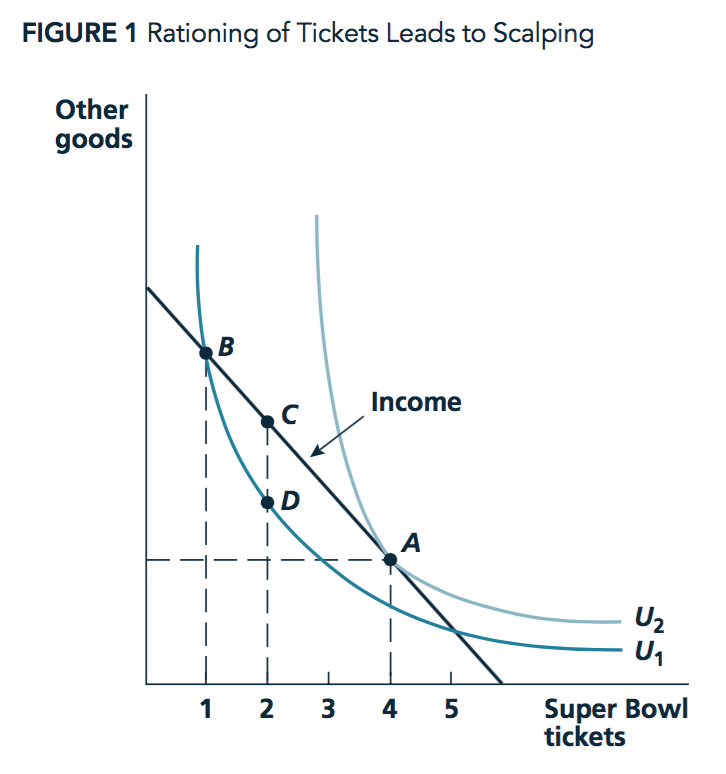
\includegraphics[width=\textwidth,height=5in]{../picsfigs/scalping.png}

{\emph{Choose TWO. Partial credit will NOT be awarded.}} Suppose the NFL
had a `rationing policy', where each consumer could buy at most one
ticket to the Super Bowl. Suppose the diagram above represents each
consumer's budget constraint and two of her indifference curves. The
maximum amount she would be willing to pay to buy an additional (second)
ticket is characterised by the vertical distance between
(\_\_\_\_\_\_\_\_\_\_\_\_\_\_)

and

(\_\_\_\_\_\_\_\_\_\_\_\_)

(choose two):

\begin{enumerate}
\def\labelenumi{\Alph{enumi}.}
\item
  A
\item
  B
\item
  C
\item
  D
\end{enumerate}

Ans: B and D

Discussion: Paying an additional amount equal to the vertical distance
between B-D (giving up this amount of `other goods') and obtaining a
second ticket would put her at point D. This point leaves her as well
off as the point she was at before, point B. Thus this is the
\emph{most} she would pay for the second ticket.

\hypertarget{section-5}{%
\subsubsection{}\label{section-5}}

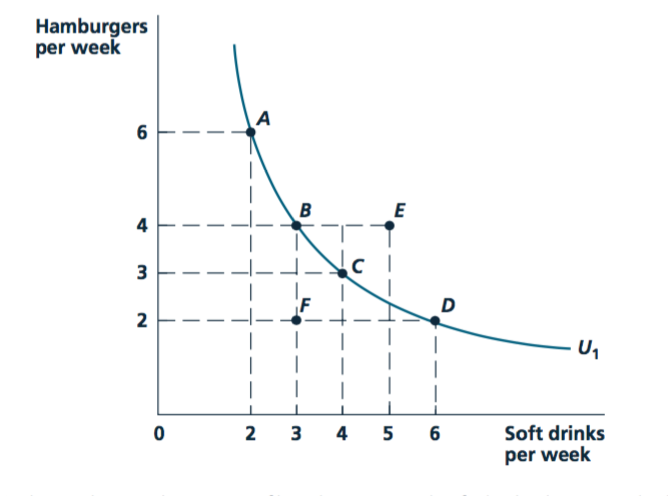
\includegraphics[width=\textwidth,height=4in]{../picsfigs/fig2-2.png}

\emph{(Choose all that are correct, and no more.)} Considering the above
indifference curve, which of the following are true?

\begin{enumerate}
\def\labelenumi{\Alph{enumi}.}
\item
  At point A she is willing to give up approximately 2 hamburgers to
  gain 1 soft drink.
\item
  At point D she is willing to give up more than one hamburger to gain
  one soft drink.
\item
  For this consumer, these goods are perfect complements, although not
  at a 1-1 ratio.
\item
  This consumer would strictly prefer to consume at point C than to
  consume at point A.
\item
  The indifference curve demonstrates an \emph{diminishing} marginal
  rate of substitution between the two goods; at a higher level of
  hamburger consumption, she requires \emph{fewer} soft drinks to be
  willing to give up a hamburger.
\end{enumerate}

True statements:

\begin{enumerate}
\def\labelenumi{(\alph{enumi})}
\tightlist
\item
  At point A she is willing to give up approximately 2 hamburgers to
  gain 1 soft drink
\end{enumerate}

\emph{and}

\begin{enumerate}
\def\labelenumi{(\alph{enumi})}
\setcounter{enumi}{4}
\tightlist
\item
  The indifference curve demonstrates an \emph{diminishing} marginal
  rate of substitution between the two goods; at a higher level of
  hamburger consumption, she requires \emph{fewer} soft drinks to be
  willing to give up a hamburger.
\end{enumerate}

\hypertarget{section-6}{%
\subsubsection{}\label{section-6}}

If, starting from any level of consumption (with a positive consumption
of plankton), a individual can hold her utility constant by reducing her
consumption of plankton by 1 and increasing her consumption of algae by
10, then, for this individual, algae and plankton are (select only one):

\begin{enumerate}
\def\labelenumi{\Alph{enumi}.}
\item
  perfect substitutes
\item
  perfect complements
\item
  complements (but not perfect complements)
\item
  substitutes (but not perfect substitutes)
\item
  inferior goods
\end{enumerate}

perfect substitutes.

\emph{Note}: remember that perfect substitutes require the MRS to be a
\emph{constant} ratio, but that ratio need not be 1:1.

\textbf{DEMAND, ITS DERIVATION AND ITS PROPERTIES}

\hypertarget{section-7}{%
\subsubsection{}\label{section-7}}

\emph{(Choose all that are correct, and no more.)}
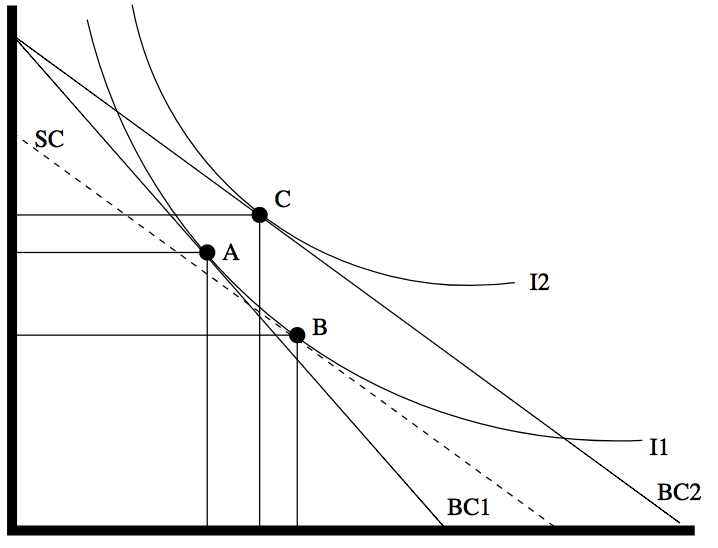
\includegraphics[width=\textwidth,height=4in]{../picsfigs/pricechangeneteffect.png}

The diagram above depicts two of an individual's indifference curves and
depicts her budget constraint before and after a price decrease, as well
as the compensated budget constraint at the initial point. For this
individual, within this range of prices, and for this income level, we
know that good X (\emph{Clarification: good X is the good depicted on
the horizontal axis}) can be classified as:

\begin{enumerate}
\def\labelenumi{\Alph{enumi}.}
\item
  a normal good
\item
  an inferior good
\item
  a Giffen good
\item
  a useless good
\item
  a luxury good
\end{enumerate}

an inferior good

\emph{Discussion:} The movement between the choice made given the
(hypothetical) budget constraint SC and the actual `new' budget
constraint BC2 depicts the income effect of the price change. Note that
this movement is the same as would occur from an increase in income
given the new price ratio.

Over this range we see that this `hypothetical increase in income' leads
to a decrease in consumption of the X good... the horizontal movement
from B to C. Thus in this range it's an inferior good. Note that as it's
inferior it cannot be normal or luxury.

However, the net effect of decrease in the price of the X good
(including substitution and income effects) is the movement from A to C.
This is an \emph{increase} in the consumption of the X good, so it is
not Giffen. (The substitution effect outweighed the income effect.)

The x good is not `useless' as the indifference curves are not
horizontal.

\hypertarget{section-8}{%
\subsubsection{}\label{section-8}}

{\emph{Choose ONE.}} Which of the following functional forms for utility
suggests the greatest substitution effect of a 0.20 increase in the
price of X when starting from the point where \(P_X =P_Y-0.10\)?

\begin{enumerate}
\def\labelenumi{\Alph{enumi}.}
\item
  \(U(X,Y) =2X+2Y\)
\item
  \(U(X,Y) = XY\)
\item
  \(U(X,Y) = 2 \times min(X,Y)\)
\item
  \(U(X,Y)=X^4Y^3\)
\item
  \(U(X,Y)=Y\)
\end{enumerate}

\(U=2X+2Y\) ~

\emph{Discussion:} This is a challenging question.

We can rule out some of these immediately.

\(U(X,Y)=Y\) implies only good Y is valued, so no substitution is
possible... and in fact the price change in X will have no impact

\(U(X,Y) = 2 \times min(X,Y)\) represents perfect complements (at ratio
A.1); we know there is no substitution effect here as there is only a
\emph{single} point (the vertex of the L-shaped indifference) curve that
yields a particular level of utility at the minimum cost.

Choice (a) \(U(X,Y) =2X+2Y\) stands out. This is `perfect substitutes'
(here at ratio 1:1) . For this case the consumer chooses the good with
greater `bang for the buck' (MU/p). Either this `better BftB' is the
same before and after the price change (in which case there's no
change), or it switches to the other good, leading to the `maximum
possible substitution.' Here both X and Y have the same MU, so the
consumer will simply choose the cheaper one. Before the increase X was
cheaper, but afterwards Y is cheaper. \(\rightarrow\) maximum possible
substitution!

Finally, consider the utility functions \(U(X,Y) = XY\) and
\(U(X,Y)=X^4Y^3\). These are basically U-shaped (in fact they are
Cobb-douglas), so there will be \emph{some substitution effect.}
However, for these, for any positive price of each good a positive
amount of each will be consumed. (Why? Because otherwise you get
\emph{no utility}!) So the substitution will not be `a complete switch
from one good to the other.'

\hypertarget{section-9}{%
\subsubsection{}\label{section-9}}

\emph{(Choose all that are correct, and no more.)} Suppose, at a
particular consumption choice that an individual is considering, her MRS
(of cider for beer) is 2:1. That is, at this point under consideration
she is willing to give up 2 ciders to gain an extra beer. This choice is
definitely *not* \emph{optimal} \emph{if}

\begin{enumerate}
\def\labelenumi{\Alph{enumi}.}
\item
  the price of beer is less than the price of cider, and the choice
  being considered involves a positive amount of cider.
\item
  the price of beer is more than twice the price of cider, and this
  choice involves consuming both beer and cider.
\item
  the price of beer is more than three times the price of cider
\item
  there are goods that give her utility other than beer and cider.
\item
  the price of beer is exactly twice that of cider.
\end{enumerate}

NOT optimal if:

the price of beer is less than the price of cider, and the choice being
considered involves a positive amount of cider.

Nor if the price of beer is more than twice the price of cider, and this
choice involves consuming both beer and cider. (or actually, if it
involves consuming any beer)

\emph{Discussion:} At this point, at the margin (i.e., considering very
small adjustments) she values beer twice as much as cider. Thus, if this
point involves consuming both beer and cider, it can only be optimal if
the price of beer is twice that of cider. If the relative price of
beer:cider is less than 2:1 she should move towards consuming more beer
and less cider. If the relative price appears more than this, she should
move towards consuming less beer and more cider.

However, if the price of beer is less than twice that of cider and she
is consuming no cider than this still may be optimal as she cannot
consume `less than zero cider'.

Similarly, if the price of beer is more than twice that of cider and she
is consuming no beer than this still may be optimal as she cannot
consume `less than zero beer'.

~\\

\emph{Remember} to read the questions carefully; note that this question
is asking for conditions such that a particular choice is \emph{NOT}
optimal.

\hypertarget{section-10}{%
\subsubsection{}\label{section-10}}

\emph{(Choose ONE)} Suppose the economy consists of five consumers, each
of whom have an individual demand curve for figs equal to
\(q_d(p) = 10-p\). Which of the following represents the \emph{market
demand} for figs:

\begin{enumerate}
\def\labelenumi{\Alph{enumi}.}
\item
  \(Q_d = 10-p\)
\item
  \(Q_d = 10-p\)
\item
  \(Q_d = 50-5p\)
\item
  \(Q_d = 50-p\)
\item
  \(Q_d = 50\)
\end{enumerate}

\(Q_d = 50-5p\)

\emph{Discussion:} we simply sum the demand curves `horizontally' ...
I.e., at every price add the quantity demanded by each of the five
consumers, so \(Q_d = 5 \times q_d(p) = 5 \times(10-p) = 50-5p.\)

\hypertarget{section-11}{%
\subsubsection{}\label{section-11}}

\emph{(Choose all that are correct, and no more.)} Which of the
following will NOT \emph{shift} the market demand curve for good X,
\(Q^{d}(X)\)?

\begin{enumerate}
\def\labelenumi{\Alph{enumi}.}
\item
  The price of good X rises.
\item
  The price of another good Y falls
\item
  The wealthiest 10\% of consumers see their income fall by £10,000
  each, while the least wealthy 90\% of consumers see their income rise
  by £10,000 each, leading to no change in total income
\item
  Consumers' preference for good X changes
\item
  Costs of producing good X fall, shifting the supply curve
\end{enumerate}

\emph{Correct choices = things that will NOT shift \(Q^{d}(X)\)}:

(a) The price of good X rises -- NO, this represents a movement along
the demand curve for X AND

(e) Costs of producing good X fall, shifting the supply curve -- NO the
shift in the supply curve doesn't enter into the market demand curve

\emph{Incorrect choices = things that will or might shift \(Q^{d}(X)\)}:

The price of another good Y falls: if the goods are complements then
\(Q^{d}(X)\) will shift out--- more quantity of X demanded at every
price \(P_X\). If the goods are substitutes than \(Q^{d}(X)\) will shift
inwards.

The wealthiest 10\% of consumers... : as we've noted even if average
income does not change a shift in the composition of income may impact
the demand curve... Here we see a redistribution of income towards the
wealthy. If X is a luxury good (in the relevant range) this should shift
the demand curve outwards; if it's a necessity (or even more extreme, an
inferior good) this will shift it inwards.

Consumers' preference for good X changes: Obviously this shifts the
demand curve

\hypertarget{section-12}{%
\subsubsection{}\label{section-12}}

\emph{(Choose ONE)} Should a price-setting firm ever set its price at a
point where demand is inelastic? Why or why not?

\begin{enumerate}
\def\labelenumi{\Alph{enumi}.}
\item
  Yes, because if demand were elastic, a rise in price would reduce
  quantity and thus reduce revenue.
\item
  Yes, because revenue is maximized where demand is the most inelastic.
\item
  No, because if it were at such a point, it could lower its price and
  its revenue would increase and costs would decline.
\item
  No, because if it were at such a point, it could raise its price and
  its revenue would increase and costs would decline.
\end{enumerate}

No, because if it were at such a point, it could raise its price and its
revenue would increase and costs would decline.

\emph{Discussion:} With inelastic demand, at the margin, a price
increase of some percentage will cause a smaller percentage decrease in
quantity demanded, and thus a rise in revenue. As less is needed to be
produced, cost will also decline.

\hypertarget{section-13}{%
\subsubsection{}\label{section-13}}

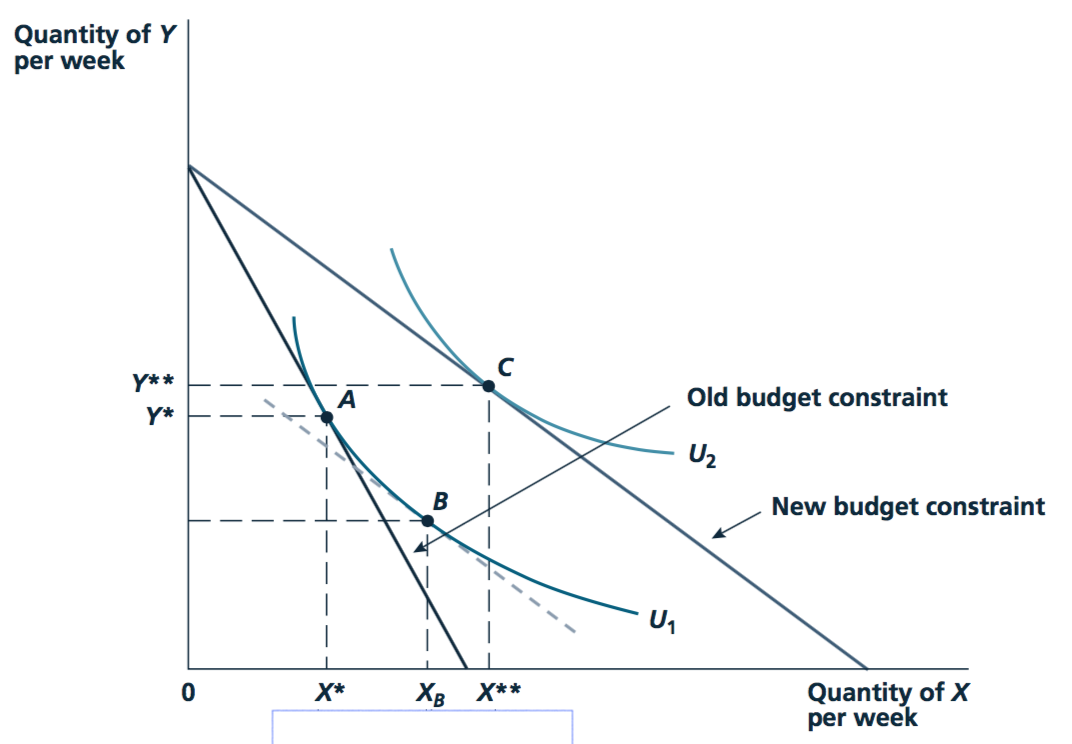
\includegraphics[width=\textwidth,height=4in]{../picsfigs/subst_income_effects.png}

\emph{Choose TWO. Partial credit will NOT be awarded for this question.}
In the graph above, the price of X has decreased, yielding the `new
budget constraint.' The \emph{income} effect of this price change (on X)
is the movement between points (choose TWO):

\begin{enumerate}
\def\labelenumi{\Alph{enumi}.}
\item
  0
\item
  \(X^{\ast}\)
\item
  \(X_B\)
\item
  \(X^{\ast\ast}\)
\item
  \(Y^{\ast}\)
\end{enumerate}

\(X_B\) and \(X^{\ast\ast}\)

\emph{Discussion:} This is straight out of the web book and textbook.

\textbf{PRODUCTION FUNCTIONS AND COSTS}

\hypertarget{section-14}{%
\subsubsection{}\label{section-14}}

Suppose MPL = 20 and MPK = 40 and the rental rate on capital is £10. If
the level of production is currently efficient (and both capital and
labour are used, with an everywhere-diminishing MRTS), the wage rate
must be

\begin{enumerate}
\def\labelenumi{\Alph{enumi}.}
\item
  £10
\item
  £5
\item
  £20
\item
  £40
\end{enumerate}

b: 5 pounds. The MRTS must equal the price ratio. Thus \(MPL/MPK=w/r\)
so here \(20/40=5/10\)

\hypertarget{section-15}{%
\subsubsection{}\label{section-15}}

\emph{(Choose all that are correct, and no more.)} Suppose the
production function for good q is given by \(q(K,L) = 3K + 2L\) where K
and L are capital and labour inputs.

Which of the following statements are true?

Consider three statements about this function:

\begin{enumerate}
\def\labelenumi{\Alph{enumi}.}
\item
  The function exhibits constant returns to scale.
\item
  The function exhibits increasing returns to scale.
\item
  The function exhibits diminishing marginal productivity for each input
  (holding the other input constant).
\item
  The function exhibits constant marginal productivities for each input
  (holding the other input constant).
\item
  A positive amount of both inputs are required to produce a positive
  output.
\end{enumerate}

The function exhibits constant returns to scale (doubling K and L
doubles outputs, for example

*and*

The function exhibits constant marginal productivities for each input:
output increases at rate 2 per labour input and at rate 3 per capital
input

\hypertarget{section-16}{%
\subsubsection{}\label{section-16}}

\emph{(Choose all that are correct, and no more.)} Which of the
following statements are correct, regarding a firm's cost curve?

\begin{enumerate}
\def\labelenumi{\Alph{enumi}.}
\item
  Total costs are the sum of fixed and variable costs
\item
  Economists include consumer surplus in their definition of revenues.
\item
  If Average Cost (AC) increases in quantity, the Average Cost (AC)
  curve must be above the Marginal Cost (MC) curve for each level of
  output.
\item
  The MC curve intersects the AC curve at its maximum (if a maximum
  exists).
\item
  If marginal costs are increasing and there are no fixed costs, this
  implies increasing AC everywhere.
\end{enumerate}

TRUE: Total costs are the sum of fixed and variable cost

If marginal costs are increasing and there are no fixed costs, this
implies increasing AC everywhere.

The others are false. Consumer surplus is not a part of revenue, it's an
entirely different thing.

If Average Cost (AC) increases in quantity, the Average Cost (AC) curve
must be BELOW the Marginal Cost (MC) curve for each level of output.

The MC curve intersects the AC curve at its MINIMUM (if a MINIMUM
exists). ... AC could be everywhere above MC if there is a fixed cost.

\textbf{Profit maximisation and supply, Perfect competition, general
equilibrium and efficiency}

\hypertarget{section-17}{%
\subsubsection{}\label{section-17}}

\emph{(Choose ONE.)} Suppose the market demand curve for a good follows
\(Q_D = 100 - P\) and the market supply follows \(Q_S = -10 + P\). What
is the total \emph{revenue} of firms (expenditure of consumers) on this
product, in equilibrium?

\begin{enumerate}
\def\labelenumi{\Alph{enumi}.}
\item
  -45
\item
  -1000
\item
  -2475
\item
  -3025
\item
  None of the above.
\end{enumerate}

100-P = P-10 \(\rightarrow\) 2p = 110 \(\rightarrow\) P=55
\(\rightarrow\) Q =

100-55=55-10=45. Revenue = Q*P = 45*55 =2475

\hypertarget{section-18}{%
\subsubsection{}\label{section-18}}

\emph{(Choose ONE.)} Under perfect competition, if an industry is
characterized by positive economic profits in the short run

\begin{enumerate}
\def\labelenumi{\Alph{enumi}.}
\item
  firms will leave the market in the long run and the short-run supply
  curve will shift outward.
\item
  firms will enter the market in the long run and the short-run supply
  curve will shift outward.
\item
  firms will enter the market in the long run and the short-run supply
  curve will shift inward.
\item
  firms will leave the market in the long run and the short-run supply
  curve will shift inward.
\end{enumerate}

b: firms will enter the market in the long run and the short-run supply
curve will shift outward.

\hypertarget{section-19}{%
\subsubsection{}\label{section-19}}

\emph{(Choose all that are correct, and no more.)} Markets can fail to
achieve efficiency for the following reason(s)

\begin{enumerate}
\def\labelenumi{\Alph{enumi}.}
\item
  There are prices consumers do not think are fair.
\item
  There are wages workers do not think are fair.
\item
  Trade puts people out of work.
\item
  There are barriers to entry, leading to monopolies.
\item
  There are too many consumers.
\end{enumerate}

e. There are barriers to entry, leading to monopolies.

\textbf{PUBLIC GOODS}

\hypertarget{section-20}{%
\subsubsection{}\label{section-20}}

\emph{(Choose all that are correct, and no more.)} Which of the
following are most reasonably considered public goods?

\begin{enumerate}
\def\labelenumi{\Alph{enumi}.}
\item
  Clothing
\item
  A giant wedge of cheese
\item
  Headache medicines provided to individuals for free by the NHS
\item
  Useful and interesting knowledge generated from an archeological
  discovery
\item
  An earthquake-prevention system that successfully prevents earthquakes
  from occuring
\end{enumerate}

Correct: Useful and interesting knowledge generated from an
archeological discovery Correct: An earthquake-prevention system that
successfully prevents earthquakes from occuring

Both of these are reasonably considered nonrival and nonexcludable, ergo
Public Goods.

\textbf{END OF PAPER}


\end{document}
